\chapter{Antecedentes}
\label{chap:antecedentes}

\drop{E}{n} este capítulo se presentarán todos los conceptos necesarios para comprender el proyecto que se va a llevar a cabo, tanto los elegidos para la realización del mismo como otros que se consideran relevantes para una correcta comprensión del problema.

Se explican también los proyectos existentes en el mercado relacionados de una forma u otra con la problemática que se quiere atajar en este \ac{TFG}, justificando la necesidad del mismo. En el mercado se pueden encontrar distintas aplicaciones y dispositivos que pueden tener una relación con el objetivo principal del presente proyecto, la mejora de la seguridad en grupos de expedición.

\section{Microcontroladores}

Un microcontrolador \cite{16} es un pequeño computador embebido en un chip, que por regla general incluye un microprocesador o \ac{CPU}, una cierta cantidad de memoria \acs{RAM}, memoria \acs{ROM} y elementos de conversión de señal analógica a digital y viceversa. También suele incluir elementos de control de entrada/salida además de ge1neradores de señales y \textit{timers}.

Los microcontroladores se usan para ejecutar pequeñas tareas específicas y normalmente se encuentran embebidos en algún otro disposivo. Estas tareas pueden ser el control de algún dispositivo como una cámara de vídeo, o de alguna funcionalidad concreta dentro de un coche, por ejemplo.

\begin{figure}[!h]
\begin{center}
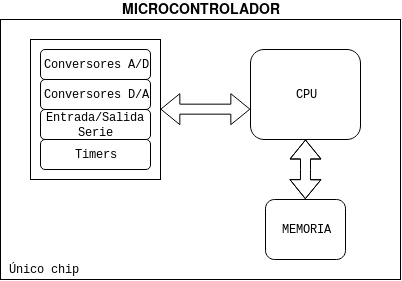
\includegraphics[width=0.4\textwidth]{microcontrollers.png}
\caption{Esquema de un microcontrolador.}
\label{fig:microcontrolador}
\end{center}
\end{figure}

\subsection{Arduino}

Arduino \cite{18} es una placa de computación física de código abierto, para crear prototipos interactivos programados de una manera fácil e intuitiva. Debido a su naturaleza de código abierto, posee una gran comunidad que comparte sus diseños, por lo que aprender a usar Arduino resulta más sencillo, siendo su curva de aprendizaje relativamente leve, si la comparamos con otros microcontroladores.

La placa de Arduino \cite{17} consiste en un microprocesador \texttt{ATmega328}. La placa contiene varios pines de entrada/salida, tanto analógica como digital, que servirán para conectar distintos tipos de sensores y actuadores.

Para programar Arduino, se usa Arduino IDE\footnote{\url{https://www.arduino.cc/en/Main/Software}}, un entorno de desarrollo gratuito que permite programar \textit{software} en un lenguaje que Arduino comprende. Este lenguaje está basado en los lenguajes de programación C y C++ y se puede extender usando librerías programadas en C++. Usando este \textit{\ac{IDE}}, se puede cargar un \textit{software} determinado en la placa Arduino de una manera muy sencilla.

Que la curva de aprendizaje de Arduino sea más leve que la de otros microcontroladores \cite{9}, no quiere decir que Arduino sea una peor alternativa que todos ellos, ya que la capa de \textit{hardware} trabaja con el mismo nivel de sofisticación que otros dispositivos embebidos. Se suele elegir Arduino cuando se quiere un desarrollo rápido y obtener facilidades en la implementación.

El esquema básico de un código Arduino se puede observar en el listado \ref{lst:basicard}. Arduino siempre posee las funciones \texttt{setup} y \texttt{loop}. La función \texttt{setup} se usa para inicializar el estado del programa. Este código se ejecuta sólo una vez al inicio del programa. La función \texttt{loop}, contiene el código principal del programa y se ejecuta de forma continua. Un programa en Arduino no puede acabar, se ejecutará de forma ininterrumpida mientras la placa esté encendida. Tampoco es posible ejecutar más de un programa en paralelo en Arduino.

\begin{lstlisting}[language=c++,captionpos=t,caption={\textbf{Esquema básico de un código Arduino.}},label={lst:basicard}]
void setup() {
}
void loop() {
}
\end{lstlisting}

\paragraph{Ventajas de usar el microcontrolador Arduino.}

Las principales ventajas en el uso de Arduino se pueden contemplar a continuación:


\begin{enumerate}[]
\item Facilidad de configuración. Arduino es un dispositivo \textit{plug-and-play}, por lo que el tiempo de configuración es mínimo.
\item Integración con una gran cantidad de sensores. Muchos de los sensores que se van a usar en este proyecto, poseen librerías para interactuar con Arduino, por lo que se produce un ahorro de tiempo en la creación y uso de estas bibliotecas.
\item El \textit{hardware} es de bajo coste. Como este proyecto es una red de dispositivos, tiene sentido crear varios prototipos e interconectarlos, en vez de uno solo. El prototipo tenía que ser, por tanto, lo más barato posible.
\item La programación del \textit{software} se realiza en un lenguaje basado en C y C++, lenguajes conocidos por el estudiante. 
\end{enumerate}

\subsection{Raspberry Pi}

Raspberry Pi es un microcontrolador \cite{19}, lanzado al mercado por la Fundación Raspberry Pi\footnote{\url{https://www.raspberrypi.org}}. Existen varias versiones de este microcontrolador pero todas tienen en común el bajo precio del mismo, en torno a los 30 euros. Raspberry Pi puede ejecutar aplicaciones sobre un sistema operativo, al contrario que Arduino, que ejecuta directamente el \textit{software} sobre el \textit{hardware}. 

Raspberry Pi tiene un microprocesador \texttt{ARM} y un juego de instrucciones \ac{RISC} de 32 bits hasta la versión \texttt{Raspberry Pi3}. Desde esta versión en adelante usa un juego de instrucciónes \ac{RISC} de 64 bits. También posee una \textit{\ac{GPU}} y memoria \ac{SDRAM}.

\begin{figure}[!h]
\begin{center}
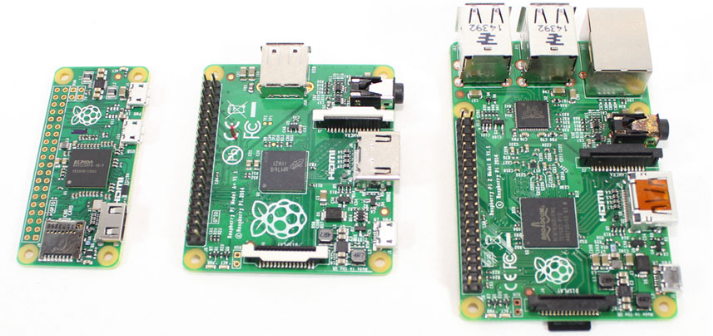
\includegraphics[width=0.6\textwidth]{raspberries.png}
\caption[]{Varios modelos de Raspberry Pi. \texttt{Raspberry Pi Zero}, \texttt{Raspberry Pi A+} y \texttt{Raspberry Pi2} (de izquierda a derecha). \protect\footnotemark}
\label{fig:raspberries}
\end{center}
\end{figure}

\footnotetext{Imagen original extraída de \cite{21}}


Raspberry Pi fue lanzado con el propósito de enseñar a programar \cite{21}, sin embargo es una gran plataforma para entusiastas del \textit{hardware}, que buscan un dispositivo para sus proyectos de electrónica. Raspberry Pi posee una serie de pines, denominados <<\textit{\ac{GPIO}} \textit{pins}>> que proporcionan una interfaz de comunicación con distintos sensores y actuadores. Dependiendo de la versión de Raspberry Pi el número de <<\ac{GPIO} \textit{pins}>> puede variar. 

Se pueden instalar muchos sistemas operativos en Raspberry Pi, pero sin duda el más usado es \texttt{Raspbian}, un sistema operativo basado en \texttt{Debian}. El sistema operativo se <<\textit{flashea}>> en una tarjeta de memoria \ac{SD}, que se introducirá en la Raspberry. A partir de esta tarjeta \ac{SD}, se puede iniciar el sistema operativo.

El principal lenguaje para programar una Raspberry Pi es Python\footnote{\url{https://www.python.org}} \cite{20}, aunque también se pueden usar otros lenguajes como C++, C o Java. Python es uno de los lenguajes más populares hoy en día y además tiene una curva de aprendizaje mucho menos pronunciada que otros lenguajes como C o C++. Además, existen un gran número de librerías para Python, lo que supone un ahorro de tiempo a la hora de la programación. El Listado \ref{lst:rasppy} muestra cómo encender y apagar un led, usando Python como lenguaje de programación.

\begin{lstlisting}[language=python,captionpos=t,caption={\textbf{Encender y apagar un led en Raspberry.}},label={lst:rasppy}]
import RPi.GPIO as GPIO
import time

GPIO.setmode(GPIO.BCM)
GPIO.setup(18, GPIO.OUT)  # Estblecer pin 18 como salida
 
while True:
  GPIO.output(18, 1)      # Encender pin 18
  time.delay(1)       
  GPIO.output(18,0)       # Apagar pin 18
\end{lstlisting}

\subsection{Otros microcontroladores}

\begin{enumerate}
\item \textbf{mbed}. \\
La plataforma \texttt{mbed}\footnote{\url{https://www.mbed.com/en/}} \cite{22} es similar a Arduino en lo que a objetivos se refiere, pero está más orientado a la prototipación sobre una placa. Usa una arquitectura basada en un microprocesador \texttt{ARM Cortex-M3}, mucho más potente que otros microprocesadores, como el \texttt{ATmega328} de Arduino. 

\texttt{mbed} posee un gran número de librerías, ya que existe una gran comunidad de programadores para esta plataforma. Para desarrollar para el microcontrolador \texttt{mbed}, no es necesario descargar \textit{software} adicional, puesto que todas las herramientas se pueden encontrar online.

\begin{figure}[!h]
\begin{center}
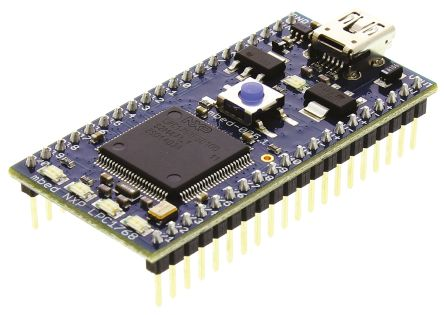
\includegraphics[width=0.4\textwidth]{mbed.jpg}
\caption[]{Microcontrolador \texttt{mbed}. \protect\footnotemark}
\label{fig:mbed}
\end{center}
\end{figure}

\footnotetext{Imagen extraída de \url{https://media.rs-online.com/t_large/R7039238-01.jpg}}

Para subir un programa compilado a la placa tan sólo hay que conectarla por \ac{USB} al computador. El código se copiará en la placa y, después de presionar el botón de \textit{reset}, la placa estará lista para ejecutar el programa que se ha desarrollado.

Al igual que con Arduino, no se puede acceder al código final generado por el compilador, para optimizarlo en caso de ser necesario. No hay herramientas de depuración para \texttt{mbed}.

\item \textbf{STM32}

\texttt{STM32} es un microcontrolador desarrollado por la compañía \textit{ST Microelectronics} \cite{23}. Existen varios \textit{kits} de \texttt{STM32} pero todos tienen en común el bajo coste de los mismos, en torno a 15 dólares. Las placas \texttt{STM32} pueden ser programadas usando código ensamblador o con el lenguaje de programación C.

La placa \cite{24} posee un microprocesador \texttt{ARM Cortex-M3} (o \texttt{ARM Cortex-M4} en los últimos modelos) de 32 bits. Este microprocesador nos proporciona un gran rendimiento y flexibilidad, aunque existen contras como la dificultad en el desarrollo de \textit{software} para la placa \texttt{STM32} si eres principiante. Además, la placa \texttt{STM32} soporta un \ac{RTOS}, lo que supone que se pueden programar sistemas mucho más complejos que en otros microcontroladores, como Arduino.

\begin{figure}[H]
\begin{center}
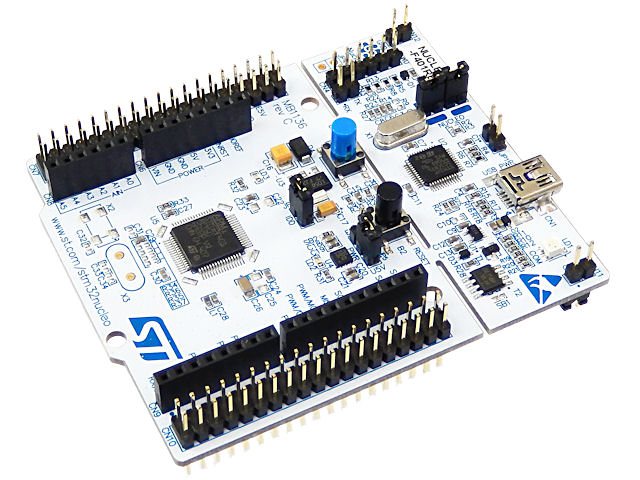
\includegraphics[width=0.4\textwidth]{nucleoSTM32.jpg}
\caption[]{Placa \texttt{STM32 Nucleo}. \protect\footnotemark}
\label{fig:stm32}
\end{center}
\end{figure}

\footnotetext{Imagen extraída de \url{https://grobotronics.com/stm32-nucleo-development-board-for-stm32-f1-series-with-stm32.html?sl=en}}

Para programar la placa \texttt{STM32}, se puede hacer uso del \textit{software} \texttt{STM32CubeMX}\footnote{\url{https://www.st.com/en/development-tools/stm32cubemx.html}}. Se trata de una herramienta de interfaz gráfica, que ayuda a crear configuraciones para la placa usando el lenguaje de programación C.  

\end{enumerate}


\begin{table}[!h]
\centering
\begin{tabular}{c|c|c|c|c|c|c|c|}
\cline{2-8}
\multicolumn{1}{l|}{}                                                                          & Procesador                                                                             & \begin{tabular}[c]{@{}c@{}}Velocidad\\ de Reloj\end{tabular} & \begin{tabular}[c]{@{}c@{}}Memoria\\ \textit{Flash}\end{tabular} & \ac{SRAM}                                                   & \ac{EEPROM} & \begin{tabular}[c]{@{}c@{}}Tarjeta\\ \ac{SD}\end{tabular} & Lenguaje                                                         \\ \hline
\multicolumn{1}{|c|}{\begin{tabular}[c]{@{}c@{}}Arduino\\ \texttt{UNO}\end{tabular}}               & \texttt{ATmega328}                                                                     & $16$ MHz                                                     & $32$ KB                                                          & $2$ KB                                                      & $1$ KB      & No                                                        & C++                                                              \\ \hline
\multicolumn{1}{|c|}{\begin{tabular}[c]{@{}c@{}}Raspberry\\ Pi 3B\end{tabular}}                & \begin{tabular}[c]{@{}c@{}}\texttt{ARM}\\ \texttt{Cortex-}\\ \texttt{A53}\end{tabular} & $1.2$ GHz                                                    & -                                                                & \begin{tabular}[c]{@{}c@{}}$1$ GB\\ \ac{SDRAM}\end{tabular} & -           & Sí                                                        & \begin{tabular}[c]{@{}c@{}}Python,\\ C, C++,\\ etc.\end{tabular} \\ \hline
\multicolumn{1}{|c|}{\texttt{mbed}}                                                            & \begin{tabular}[c]{@{}c@{}}\texttt{ARM}\\ \texttt{Cortex-M3}\end{tabular}              & $96$ MHz                                                     & $512$ KB                                                         & $32$ KB                                                     & -           & No                                                        & C, C++                                                           \\ \hline
\multicolumn{1}{|c|}{\begin{tabular}[c]{@{}c@{}}\texttt{STM32}\\ \texttt{Nucleo}\end{tabular}} & \begin{tabular}[c]{@{}c@{}}\texttt{ARM}\\ \texttt{Cortex-M4}\end{tabular}              & $84$ MHz                                                     & $512$ KB                                                         & $96$ KB                                                     & -           & No                                                        & C                                                                \\ \hline
\end{tabular}
\caption{Comparativa de las principales características de los distintos microcontroladores}
\label{table:comparacionMicros}
\end{table}

\section{Sensores}

Los sensores son \cite{25} componentes eléctricos o electrónicos que funcionan como dispositivos de entrada. No todas las entradas son explícitamente sensores, pero las entradas usan sensores. Por ejemplo, en el caso de un ratón de ordenador. El ratón no es un sensor en sí mismo, pero contiene una serie de ellos, por ejemplo el sensor que detecta el movimiento del mismo.

Podemos pensar en sensores como componentes que miden estímulos externos al sistema (miden el entorno del sistema). El sistema, puede reaccionar a estos estímulos mediante los \textbf{actuadores}. Por ejemplo, un sistema con un sensor de luminosidad, puede detectar la cantidad de luz que existe en el ambiente. Procesando esta cantidad de luz, se puede obtener como salida la activación o no de una bombilla.

Para el desarrollo de este proyecto se han usado distintos sensores, que se comentarán a continuación:

\begin{enumerate}
\item \textbf{Sensor \acf{LDR}} \\
El sensor \texttt{GL5528} es un \ac{LDR}, que consiste en una resistencia variable con respecto a la luz. La resistencia del fotoresistor decrementa conforme incrementa la intensidad de la luz sobre el mismo. 

\begin{figure}[!h]
\begin{center}
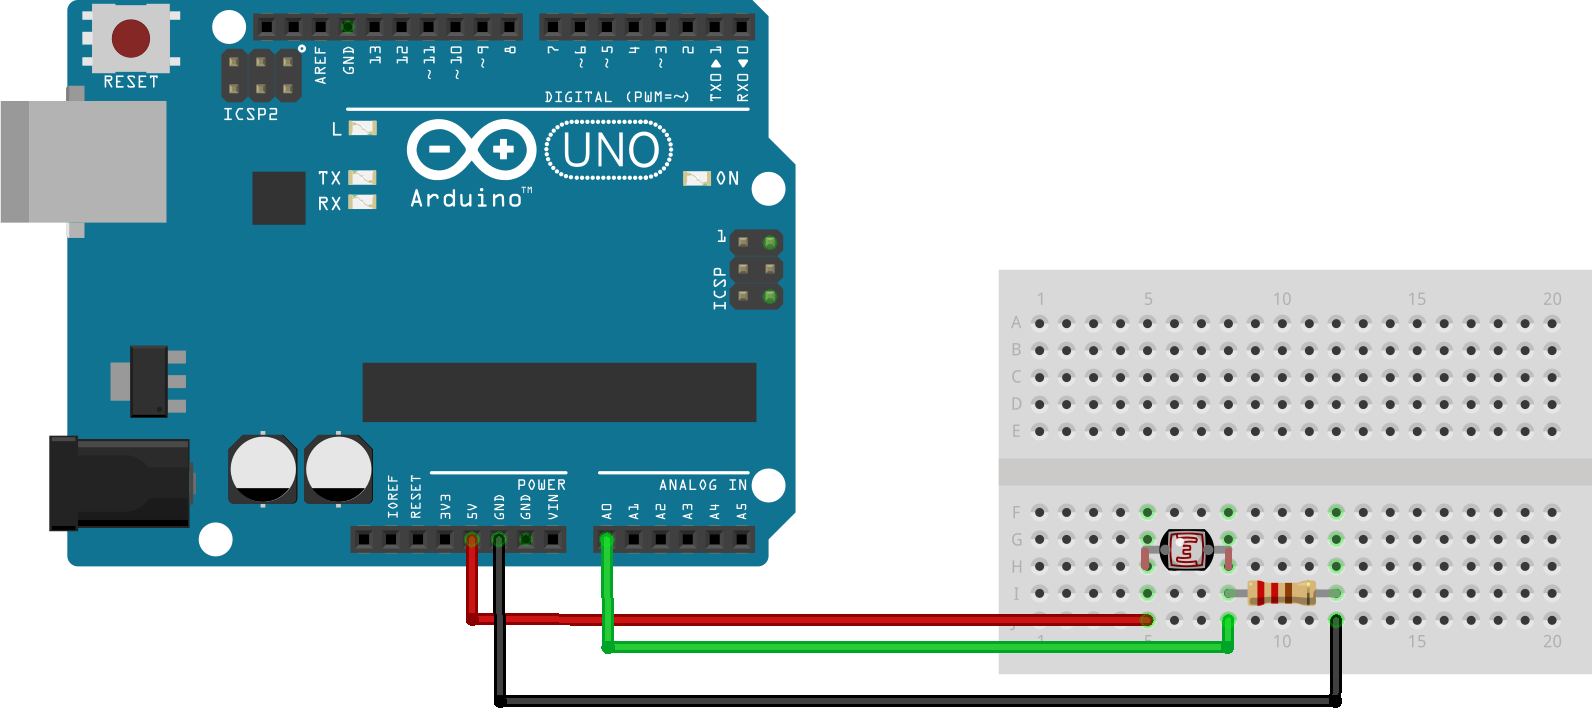
\includegraphics[width=0.6\textwidth]{ldr_esquema.png}
\caption{Esquema de conexión del \ac{LDR} y Arduino.}
\label{fig:gl5528}
\end{center}
\end{figure}

Para elegir el valor de la resistencia que acompaña al \ac{LDR}, se puede usar la fórmula de \textit{Axel Benz}. Si se usase el sensor en un área muy luminoso con una resistencia de \textit{pull-down} de $10K\Omega$, se saturará rápidamente. El votaje a través de la resistencia pronto será de $5V$ y no se podrá diferenciar con facilidad entre algo brillante y algo muy brillante. En este caso, habría que reemplazar la resistencia de $10K\Omega$ por una de $1K\Omega$, pero ahora no se detectarán los niveles de oscuridad tan bien como antes. Para encontar ese valor de resistencia, usamos la fórmula de \textit{Axel Benz}:

\begin{center}
\begin{equation}
R_{ref} = \sqrt{R_{Min} \cdot R_{Max}}
\end{equation}
\label{eq:referenceResistance}
%\myequations{Fórmula de \textit{Axel Benz}}
\end{center}

El valor $R_{Max}$, es el valor de resistencia que ofrece el \ac{LDR}, cuando se encuentra no recibe nada de luminosidad. El valor de $R_{Min}$ es el valor de resistencia que ofrece el \ac{LDR} cuando recibe la luminosidad máxima.

\begin{lstlisting}[language=c++,captionpos=t,caption={\textbf{Utilización básica del sensor GL5528.}},label={lst:basicgl5528}]
#include "GL5528.h"

GL5528 gl5528(A0);

void setup(){
 pinMode(A0, INPUT);    // Set A0 pin as an input pin
 Serial.begin(9600);
}

void loop(){  
  LightThresholds light_thres = gl5528.getLightMeasure();  
  if (light_thres == LightThresholds::LT_VERY_SUNNY)
  {
    Serial.println("Very Sunny"); 
  }
  else if (light_thres == LightThresholds::LT_NIGHT)
  {
    Serial.println("It's night");  
  }
}
\end{lstlisting}

\vspace*{0.3in}


\item \textbf{Sensor de lluvia} \\
El sensor de lluvia \texttt{YL-83} es una herramienta para la detección de lluvia. Se puede usar como un indicador que señala cuándo una gota de agua cae en la placa detectora y también para medir la intensidad de lluvia. Este sensor permite ajustar la sensibilidad a través de un potenciómetro.

Con la salida analógica se obtiene un valor que puede ser usado para detectar la intensidad de lluvia. La salida digital indica la presencia o ausencia de lluvia. 

La resistencia que posee la placa detectora varía de acuerdo a la cantidad de agua que existe en su superficie. Cuanta más agua exista en la superficie, menor será el voltaje de salida. Por tanto, un voltaje bajo de salida indica que la resistencia interna de la placa detectora ha aumentado y, por tanto, existe agua en su superficie. Un voltaje alto de salida indicará que no existe agua. Los valores intermedios se pueden usar para identificar la intensidad de la lluvia.


\begin{figure}[!h]
\begin{center}
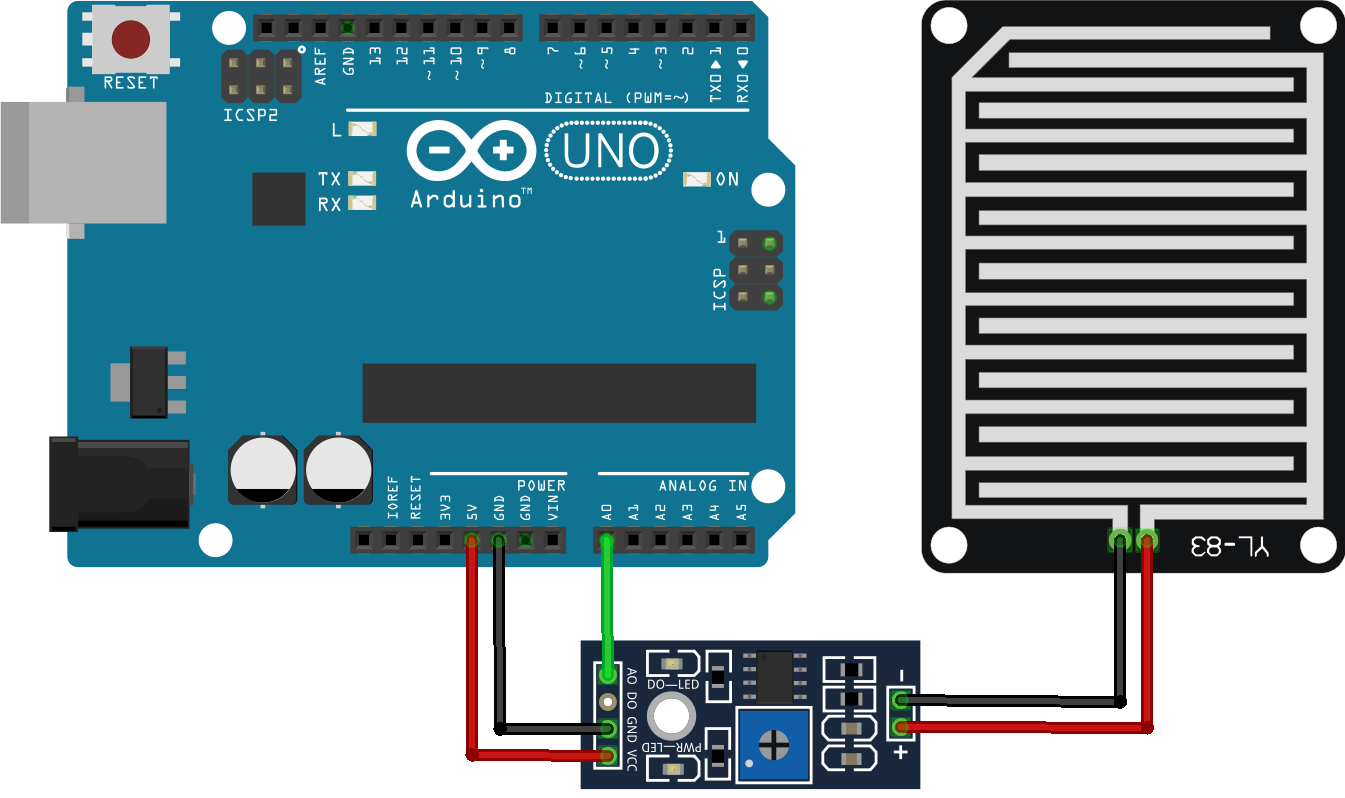
\includegraphics[width=0.6\textwidth]{rainsensor_esquema.png}
\caption{Esquema de conexión del sensor de lluvia \texttt{YL-83}.}
\label{fig:yl83}
\end{center}
\end{figure}

\begin{lstlisting}[language=c++,captionpos=t,caption={\textbf{Utilización básica del sensor de lluvia YL38.}},label={lst:basicYL38}]
#include <RainSensorYL38.h>

RainSensorYL38 RainSensor(A0);

void setup() {
  Serial.begin(9600);
}

void loop() {
  RainAmount rainamount = RainSensor.GetRainAmount();
  switch (rainamount)
  {
    case RainAmount::RA_NO_RAIN:
      Serial.println("No Rain");
      break;
    case RainAmount::RA_LOW_RAIN:
      Serial.println("Low rain");
      break;
    case RainAmount::RA_MODERATE_RAIN:
      Serial.println("Moderate rain");
      break;
    case RainAmount::RA_HEAVY_RAIN:
      Serial.println("Heavy rain");
      break;
  }
}
\end{lstlisting}

\item \textbf{Sensor de temperatura y humedad}

En este proyecto se ha usado el sensor de temperatura y humedad \texttt{DHT22} \cite{26}. Tiene un rango de medición de temperatura que va desde $-40$ hasta $125$ grados Celsius, con una precisión de $\pm0.5$ grados Celsius. En lo que a la humedad se refiere, posee un rango de medición de humedad que va desde el $0\%$ hasta el $100\%$, con una precisión de entre el $2$ y el $5\%$. El sensor \texttt{DHT22} realiza una medición cada dos segundos y opera tanto a $3V$ como a $5V$. 

Para medir la humedad, usa un componente sensible a la humedad con dos electrodos y entre ellos un substrato en el que se mantiene la humedad. Tan pronto como la humedad cambia, la conductividad del substrato cambia y también varía la resistencia entre los electrodos. Estos cambios son medidos e interpretados por el sensor.

En lo que a temperatura se refiere, el sensor usa un termistor, una resistencia variable que cambia su valor con respecto a la temperatura. Cuanto menor es la temperatura, más alta es la resistencia. La resistencia va disminuyendo conforme la temperatura aumenta. 

https://desarrollador-android.com/wp-content/uploads/2015/05/basic-lifecycle.png
\begin{figure}[!h]
\begin{center}
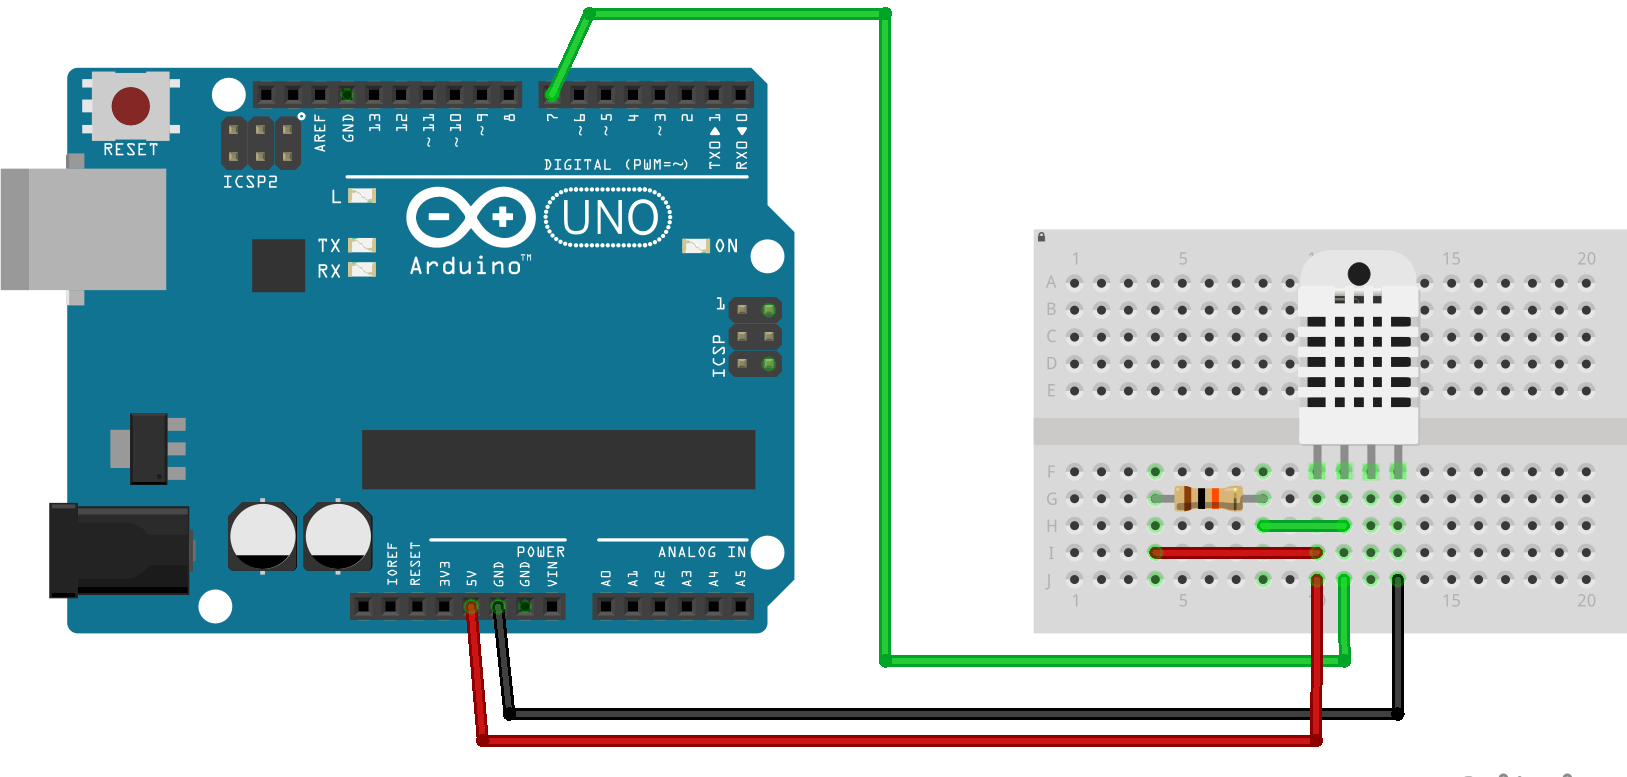
\includegraphics[width=0.6\textwidth]{temp_hum_esquema.png}
\caption{Esquema de conexión del sensor de temperatura y humedad \texttt{DHT22}.}
\label{fig:dht22}
\end{center}
\end{figure}

\begin{lstlisting}[language=c++,captionpos=t,caption={\textbf{Utilización básica del sensor de temperatura y humedad DHT22.}},label={lst:basicDHT22}]
#include <DHT22.h>

#define DHT22_PIN 7

DHT22 myDHT22(DHT22_PIN);

void setup(void)
{
  Serial.begin(9600);
}

void loop()
{ 
  DHT22_ERROR_t errorCode;
  
  delay(2000);	// The sensor need 2 seconds between readings
  
  errorCode = myDHT22.readData();
  if (errorCode == DHT_ERROR_NONE)
  {
      Serial.print("Temperature: "); Serial.print(myDHT22.getTemperatureC());
      Serial.print("C\t|\tHumidity: "); Serial.println(myDHT22.getHumidity());
  }
  else
  {
    char buffer[50];
    myDHT22.getErrorString(errorCode, buffer);
    Serial.println(buffer);
  } 
}
\end{lstlisting}

\item \textbf{Sensor de pulso cardíaco}

Para el desarrollo de este proyecto, se ha usado el sensor de pulso cardíaco \texttt{PulseSensor}\footnote{\url{https://pulsesensor.com}}. Este sensor combina un sensor de pulso cardíaco óptico, con un circuito de amplificación de señal y cancelación de ruido, lo que proporciona unas mediciones de pulso cardíaco bastante confiables. 

El sensor \texttt{PulseSensor}, es básicamente un fotopletismógrafo. Esto es, un dispositivo que utiliza un haz de luz para monitorizar, de una forma no invasiva el pulso cardíaco. Este sensor identifica instantes sucesivos en los que se produce un latido, para medir el tiempo entre ellos. Este tiempo se denomina \ac{IBI} y se puede usar para calcular el ritmo cardíaco.

\begin{figure}[!h]
\begin{center}
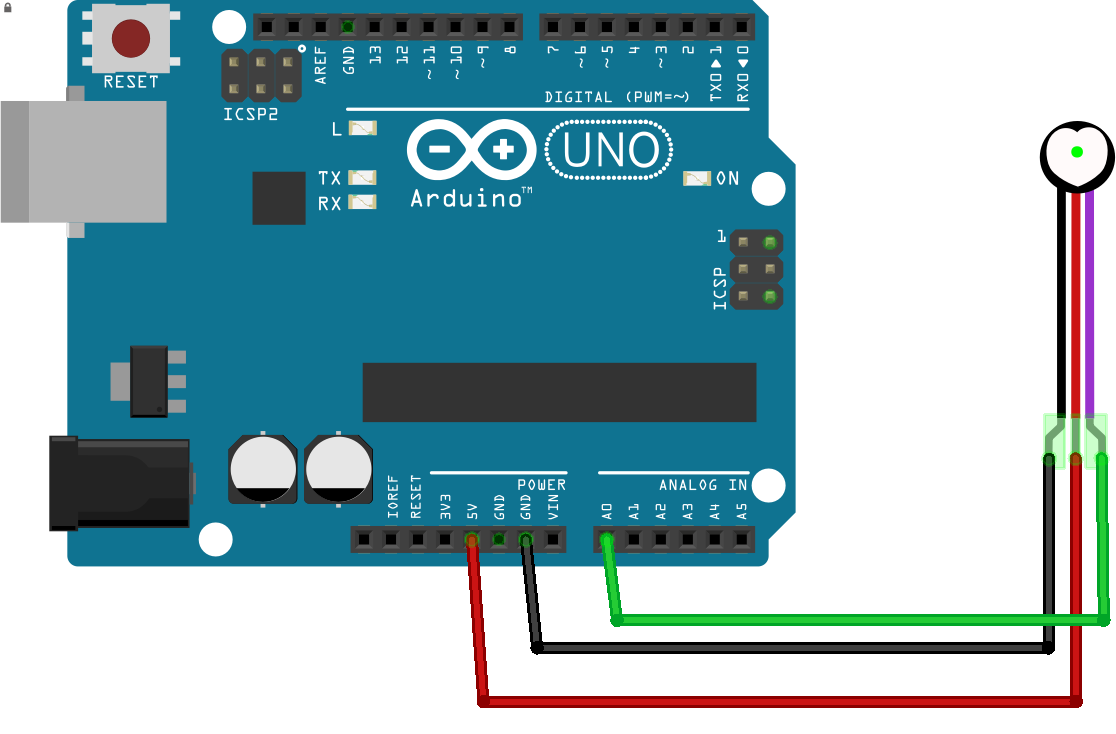
\includegraphics[width=0.45\textwidth]{pulsesensor_esquema.png}
\caption{Esquema de conexión del sensor de pulso cardíaco \texttt{PulseSensor}.}
\label{fig:pulsesensor}
\end{center}
\end{figure}

\begin{lstlisting}[language=c++,captionpos=t,caption={\textbf{Utilización básica del sensor de pulso cardíaco.}},label={lst:basicPulsesensor}]
#define USE_ARDUINO_INTERRUPTS true
#include <PulseSensorPlayground.h>

const int OUTPUT_TYPE = SERIAL_PLOTTER;
const int PULSE_INPUT = A0;
const int THRESHOLD = 550;   // Adjust this number to avoid noise when idle
PulseSensorPlayground pulseSensor;

void setup() {
  Serial.begin(115200);
  pulseSensor.analogInput(PULSE_INPUT);
  pulseSensor.setSerial(Serial);
  pulseSensor.setOutputType(OUTPUT_TYPE);
  pulseSensor.setThreshold(THRESHOLD);
}

void loop() {
  delay(100);
  // write the latest sample to Serial.
  pulseSensor.outputSample();
  if (pulseSensor.sawStartOfBeat()) 
  {
    pulseSensor.outputBeat();
  }
}
\end{lstlisting}

\item \textbf{Sensor acelerómetro y giroscopio}

Un giroscopio es un sensor que se encarga de medir la velocidad angular, o lo que es lo mismo, la velocidad de rotación de un objeto alrededor de uno de sus ejes. El giroscopio puede usarse para determinar la orientación de un cierto objeto, por ejemplo.

Un acelerómetro es un sensor diseñado para medir la aceleración no gravitacional en uno, dos o tres ejes. El acelerómetro es capaz de detectar cambios en las fuerzas que actúan sobre él, debido a un movimiento, por ejemplo. Con la variación de la velocidad, se puede calcular la aceleración del objeto. También se pueden calcular de forma indirecta otras medidas, como la velocidad y el desplazamiento de un objeto.

El sensor \texttt{MPU6050} se compone de un acelerómetro de 3 ejes y un giroscopio de 3 ejes, que permite medir aceleración y velocidad angular en el espacio tridimensional. Este sensor proporciona seis valores de salida con cada medición: aceleración en los ejes $X$, $Y$, $Z$ y velocidad angular en los ejes $X$, $Y$, $Z$.

\begin{figure}[!h]
\begin{center}
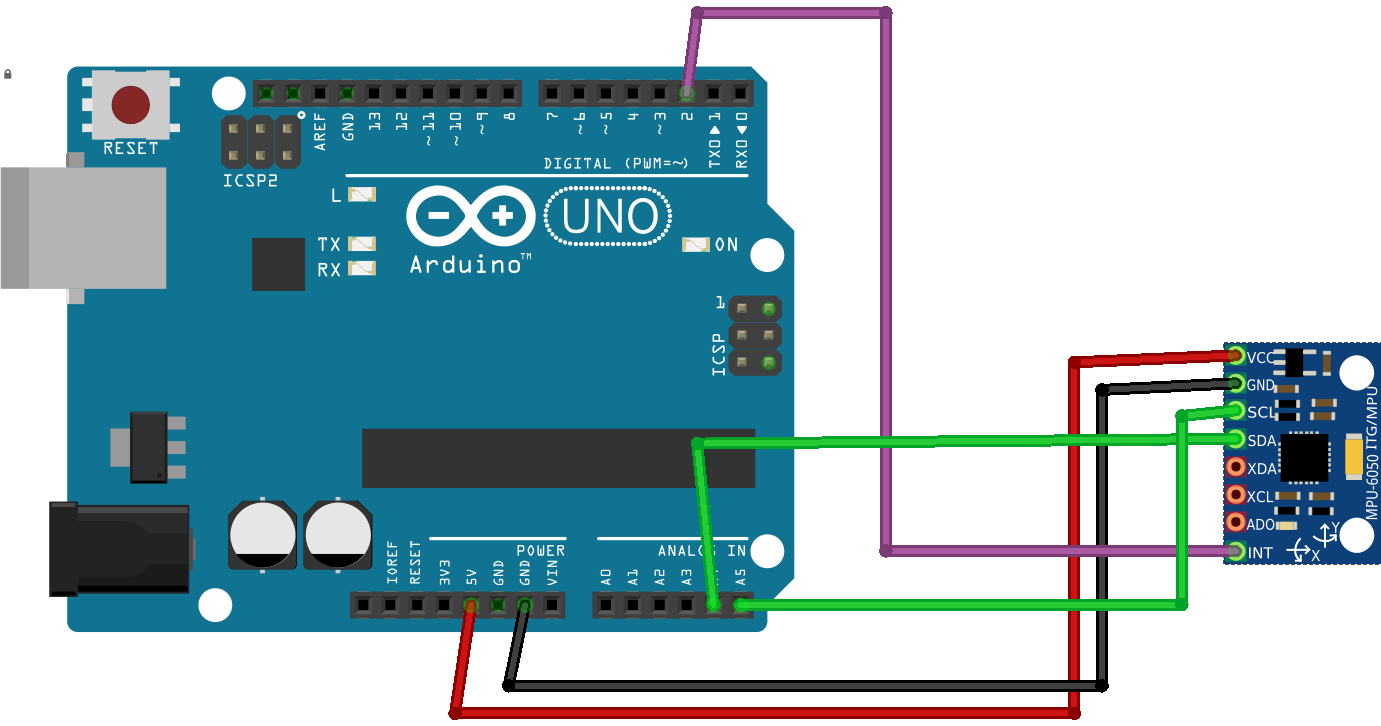
\includegraphics[width=0.6\textwidth]{giroscope_esquema.png}
\caption{Esquema de conexión del acelerómetro y giroscopio \texttt{MPU6050}.}
\label{fig:mpu6050}
\end{center}
\end{figure}
\end{enumerate}

\begin{lstlisting}[language=c++,captionpos=t,caption={\textbf{Utilización básica del acelerómetro y giroscopio MPU6050.}},label={lst:basicMPU6050}]
#include "I2Cdev.h"
#include "MPU6050.h"
#include "Wire.h"

MPU6050 sensor;

int ax, ay, az;
int gx, gy, gz;

bool initiated = false;

void setup() {
  Wire.begin();           // Initiate I2C  
  sensor.initialize();    // Initiate the sensor
  if (sensor.testConnection()) initiated = true;
}

void loop() {
  if (initiated)
  {
    // Read acceleration and angular velocity
    sensor.getAcceleration(&ax, &ay, &az);
    sensor.getRotation(&gx, &gy, &gz);
  }
  delay(100);
}
\end{lstlisting}

\section{Sistemas Operativos para Dispositivos Móviles}
\subsection{Android}

Android es un sistema operativo de código abierto, desarrollado por Google \cite{27}. Está basado en el núcleo de Linux y está diseñado principalmente para dispositivos móviles con una pantalla táctil, como pueden ser \textit{smartphones} o \textit{tablets}. Android es el sistema operativo para móviles más usado en el mundo, con más de dos mil millones de dispositivos en la actualidad. Desarrollar una aplicación para un dispositivo Android significa que cualquier dispositivo que tenga este sistema operativo será capaz de ejecutarla, sea del fabricante que sea, abstrayendo aspectos relativos a cada modelo de dispositivo. Android no solo está presente en dispositivos móviles, en los últimos años se puede observar un crecimiento de Android en televisores y otras máquinas, como pueden ser los coches.

Android es un sistema operativo que goza de varias versiones. Cada versión se compone por un número de versión, un nombre de sistema operativo y un nivel de \ac{API}. El número de versión se asemeja al sistema de versionado convencional (2.1, 4.0, 5.4.3). Si se produce un cambio en el primer dígito de la versión, el sistema operativo sufre un cambio notorio, con muchas \ac{API}s nuevas. Si cambia el segundo dígito, se produce una evolución en el sistema operativo. Si, por el contrario, es el tercer dígito de la versión el que cambia, se habrán producido cambios menores. Los niveles de la \ac{API} se numeran de forma monótona y el código de nombres asignados al sistema operativo siempre se refiere a comidas dulces.

Android es un sistema operativo compatible con versiones anterirores. Esto quiere decir que una aplicación escrita para una \textit{release} antigua se ejecutará sin necesidad de ser recompilada en una \textit{release} más moderna, pero no al revés. Por ejemplo, una aplicación compilada en un dispositivo Android 4 podrá ejecutarse en un dispositivo con Android 7 pero no viceversa ya que en Android 7 se hacen usos de llamadas a \ac{API}s que no existían en Android 4.

Para el diseño visual de una aplicación Android, se puede usar la guía de <<\textit{Material Design}>> ya que en las últimas versiones, Android sigue las pautas descritas en esta guía haciendo más fácil crear una aplicación cuyos elementos visuales estén correctamente estructurados, animados y con colores acordes.

Una aplicación Android consiste en uno o más componentes, escritos en lenguaje Java (también se puede desarrollar una aplicación Android usando lenguaje Kotlin\footnote{\url{https://kotlinlang.org}}). Estos componentes pueden ser:

\begin{enumerate}
\item \textbf{Actividades}. Estos componentes abarcan la parte visual (las vistas), del código que se encarga de mostrar los datos en estas vistas y de la respuesta a ciertos eventos de un usuario, como puede ser pulsar o arrastar un elemento de la vista.

\item \textbf{Servicios}. Son componentes que no tienen parte visual y pueden ejecutarse por un período de tiempo más prolongado que una actividad, normalmente en segundo plano. Los servicios pueden continuar ejecutándose aunque el usuario pase a usar otra aplicación.

\item \textbf{\textit{Broadcast Receiver}}. Es un componente que se encarga de responder a ciertos eventos generados en el sistema, como fallos de conectividad en la red o un aviso de batería baja. 	

\item \textbf{Proveedores de Contenido}. Se usan para compartir datos con otras aplicaciones. Se pueden usar estos proveedores de contenido para tomar datos que proporcionan ciertas aplicaciones como el calendario o los contactos. 

\item \textbf{Adaptador \textit{sync}}. Se usan para sincronizar datos desde una aplicación con servicios \textit{cloud}. 
\end{enumerate}

Una aplicación en Android no tiene un método \texttt{main} que ejecutará el código, ni un método \texttt{loop} que se ejecutará de forma contínua mientras la aplicación esté abierta. Las actividades en Android siguen un ciclo de vida (véase Figura \ref{fig:activity_lifecycle}), que es necesario comprender. Una aplicación puede encontrarse en uno de los tres estados siguientes:

\begin{enumerate}
\item \textbf{Activa}. Una aplicación se encuentra activa si es visible al usuario y se está ejecutando.
\item \textbf{Pausada}. Una aplicación se encuentra en este estado si una parte de la misma ha perdido el foco y el usuario no puede interactuar con ella. Esta situación se da cuando aparece un diálogo en la aplicación, por ejemplo.
\item \textbf{Parada.} Una aplicación se encuentra parada si su vista se encuentra totalmente oculta al usuario.
\end{enumerate}

\begin{figure}[!h]
\begin{center}
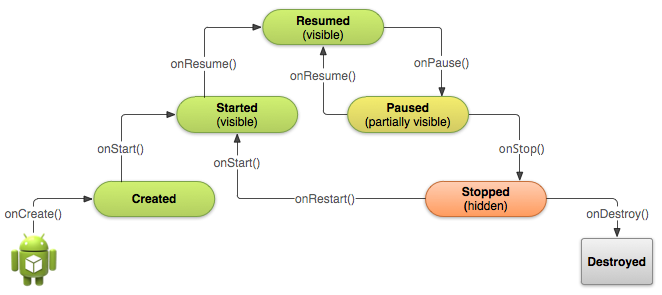
\includegraphics[width=0.6\textwidth]{activity_lifecycle.png}
\caption[]{Ciclo de vida de una actividad en Android. \protect\footnotemark}
\label{fig:activity_lifecycle}
\end{center}
\end{figure}

\footnotetext{Imagen extraída de \url{https://desarrollador-android.com/wp-content/uploads/2015/05/basic-lifecycle.png}}

Antes de comenzar a desarrollar una aplicación Android, hay que configurar la plataforma de desarrollo \cite{28}. Para realizar esto es necesario seguir una serie de pasos, como la instalación de un \ac{IDE} como es \texttt{Android Studio}, que incluye el Android \ac{SDK}. También es necesario configurar \ac{OpenJDK}, la versión libre de la plataforma de desarrollo Java.

\texttt{Android Studio} es el fruto de una colaboración entre JetBrains\footnote{\url{https://www.jetbrains.com}} y Google \cite{29}. Se ha convertido en el \ac{IDE} oficial para el desarrollo de aplicaciones Android. Este \ac{IDE} está construido sobre \texttt{IntelliJ}, por lo que la funcionalidad que aporta es un superconjunto de la que aporta \texttt{IntelliJ}. 

El \ac{AVDM} permite crear distintos \ac{AVD}, que emularán un dispositivo Android ejecutándose en el computador. El computador reserva un bloque de memoria para reproducir el entorno del dispositivo que se va a emular, es decir, se ejecuta una versión del núcleo de Linux y todo el sistema operativo Android que contendría el dispositivo físico. La emulación es mejor que la simulación, ya que proporciona un entorno más fiel al real. Sin embargo, para la creación y arranque de un \ac{AVD} se necesitan muchas más prestaciones. Para probar la aplicación Android no es necesario usar un \ac{AVD}. Si se dispone de un dispositivo Android, se puede conectar al computador para ejecutar la aplicación directamente en el dispositivo físico.

\section{Bluetooth}

Bluetooth es una forma de comunicación inalámbrica entre dispositivos a corta distancia \cite{30}. La comunicación inalámbrica existe desde finales del siglo \upperRomannumeral{19} en forma de radio, infrarojos, televisión y más recientemente el estándar 802.11. La comunicación vía Bluetooth es de corta distancia, normalmente menos de 10 metros. Tanto el \textit{hardware} como el \textit{software} están afectados por esta restricción.

Los dispositivos Bluetooth se dividen en tres clases según su potencia (en la Tabla \ref{table:bt_clas} se puede ver dicha división). La única diferencia entre esas clases es la distancia máxima de separación que puede soportar una conexión Bluetooth. La gran mayoría de dispositivos Bluetooth de hoy en día son de clase 2 (dispositivos móviles, auriculares, ratones y teclados, etc.). Existen dispositivos \ac{USB} de clase 1, que tienen mayor potencia. Si se establece una conexión entre un dispositivo de clase 1 y uno de clase 2, la distancia máxima de separación entre ellos viene dada por el dispositivo de clase 2. Los dispositivos de clase 3 son más raros, ya que tienen una fuerte limitación en el rango y los hace poco útiles.

\begin{table}[!h]
\centering
\begin{tabular}{|c|l|}
\hline
Clase & Distancia         \\ \hline
1     & 100 metros        \\ \hline
2     & 10 metros         \\ \hline
3     & \textless 1 metro \\ \hline
\end{tabular}
\caption{Clasificación de los dispositivos Bluetooth según su potencia.}
\label{table:bt_clas}
\end{table}

No es sencillo dar un dato exacto sobre la cantidad de ancho de banda en un canal de comunicaciones Bluetooth, pero teóricamente dos dispositivos Bluetooth poseen un ancho de banda asimétrico máximo de $723.2$ kbps y un ancho de banda máximo simétrico de $433.9$ kbps. Entendemos por ancho de banda asimétrico aquel en el que solo está transmitiendo un dispositivo Bluetooth y por ancho de banda simétrico aquel en el que los dos dispositivos están transmitiendo a la vez el uno al otro. Estos anchos de banda son teóricos y los reales siempre serán menores, debido principalmente al ruido en una conexión inalámbrica.

Como en todas las comunicaciones inalámbricas, la fuerza de una señal se deteriora con el cuadrado de la distancia desde el origen. Además, las señales más débiles son más fáciles de corromper por el sonido. Por tanto, el ancho de banda en una comunicación Bluetooth será menor cuanto mayor sea la distancia de separación entre los dos dispositivos. 

En la especificación Bluetooth 2.0, del año 2004, los anchos de banda aumentaron hasta $2178.1$ kbps en el caso del ancho de banda asimétrico máximo y hasta $1306.9$ kbps en el caso del ancho de banda simétrico máximo. Con la llegada de Bluetooth 3.0 en el año 2009, la velocidad máxima teórica de transferencia de datos de hasta $24$ Mbps aunque no a través del enlace Bluetooth, propiamente dicho. Si se usa la especificación Bluetooth 4.0 del año 2010, se obtienen velocidades teóricas de transferencia de datos de entre $25$ Mbps y $32$ Mbps. Con la llegada de Bluetooth 5.0 a finales del año 2016 se dobla la velocidad de transmisión de datos, además de cuadruplicar el alcance entre dos dispositivos Bluetooth.

\begin{table}[!h]
\centering
\begin{tabular}{|c|c|l|}
\hline
Año de Lanzamiento & Versión Bluetooth & \multicolumn{1}{c|}{Características introducidas}           \\ \hline
2004               & 2.0               & Velocidad de datos mejorada                                 \\ \hline
2007               & 2.1               & Emparejamiento Simple Seguro (\ac{SSP})    				 \\ \hline
2009               & 3.0               & Alta velocidad, con 802.11 Radio Wi-Fi                      \\ \hline
2010               & 4.0               & Protocolo de bajo consumo de energía                        \\ \hline
2013               & 4.1               & Conexión a dispositivos \ac{IoT} indirecta 				 \\ \hline
2014               & 4.2               & Uso de IPv6 para conexión directa a Internet                \\ \hline
2016               & 5.0               & 4 veces más rango, 2 veces más velocidad                    \\ \hline
\end{tabular}
\caption{Resumen de las características más importantes añadidas a las distintas versiones de Bluetooth.}
\label{table:bt_versions}
\end{table}

No existe un estándar sobre Internet, ya que se compone por una serie de protocolos (con sus propios estándares), como pueden ser \texttt{Ethernet}, \texttt{TCP/IP} o \ac{HTTP}. Bluetooth es parecido a Internet, ya que está compuesto también por distintos protocolos que definen por un lado las comunicaciones físicas (como las frecuencias de radio y cómo modular y demodular señales) y por otro lado otras cuestiones como por ejemplo la transmisión de audio entre dispositivos. Sin embargo, a diferencia de Internet, Bluetooth si que posee un estándar. La mayor diferencia entre Bluetooth e Internet reside en la distancia física entre dispositivos ya que en Internet la distancia no es una limitación, a priori.

En el proceso de establecimiento de una conexión Bluetooth hay un dispositivo (al que llamaremos cliente) que es quien inicia la conexión. El dispositivo servidor estará a la escucha de conexiones. Esta nomenclatura no tiene nada que ver con el modelo cliente-servidor ya que una vez establecida la conexión cualquiera de los dos dispositivos puede actuar como cliente o servidor.

Los dispositivos que quieren establecer una conexión de salida necesitan escoger un destino y un protocolo de transporte. Los dispositivos que quieren establecer conexiones de entrada necesitan escoger un protocolo de transporte y después ponerse a la escucha de conexiones de salida. Cada dispositivo Bluetooth posee un identificador único de fábrica, de 48 bits, que actúa como la dirección física. Estos identificadores no cambian nunca y son únicos por dispositivo. Como estos identificadores no son muy amigables desde el punto de vista de un usuario, se puede asignar un nombre al dispositivo Bluetooth, que el cliente se encargará de traducir a la dirección numérica. Este nombre se denomina <<nombre de exposición>>. 

Durante el descubrimiento de dispositivos, se envía un mensaje \textit{broadcast} de <<descubrimiento>>, al que otros dispositivos responden con su dirección y un número que se corresponde con el tipo de dispositivo (dispositivo móvil, PC, auriculares, etc.). El nombre de exposición se puede conocer preguntando directamente a un dispositivo concreto.

Dependiendo de las necesidades concretas de la aplicación, se puede elegir un protocolo de transporte u otro. Bluetooth posee varios protocolos de transporte a escoger, como son \ac{RFCOMM}, \ac{L2CAP}, \ac{ACL} y \ac{SCO}. De entre ellos, el protocolo más usado es \ac{RFCOMM}.

Para que puedan existir varias aplicaciones usando un mismo dispositivo Bluetooth, se usan los puertos. Varias aplicaciones, con un uso específico, poseen su número de puerto fijado. Así surgen los <<\textit{well-known ports}>>. Para conocer en qué puerto escucha una determinada aplicación a la que se quiere conectar se usa el \ac{SDP}. Todo dispositivo Bluetooth mantiene un servidor \ac{SDP} que está a la escucha en un puerto reservado (el puerto 1 en este caso). Cuando una aplicación se ejecuta en un puerto, registra una descripción y un número de puerto en el \ac{SDP}. Si una aplicación remota quiere acceder a ella, lo hará consultando al \ac{SDP}.

\begin{figure}[!h]
\begin{center}
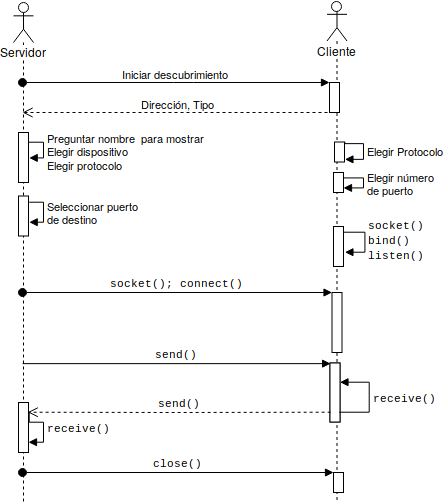
\includegraphics[width=0.6\textwidth]{bt_seq.png}
\caption{Establecimiento de una conexión Bluetooth.}
\label{fig:seq_bt}
\end{center}
\end{figure}

Los clientes necesitan saber cuál de las aplicaciones registradas en un \ac{SDP} es la que está buscando. La forma más fácil de saberlo es asignar a cada servicio un identificador único o \ac{UUID} de 128 bits. \ac{SDP} denomina a estos \ac{UUID} identificadores de servicio. Cuando una aplicación se ejecuta quedando a la espera de conexiones Bluetooth, registra en el \ac{SDP} su identificador de servicio. Una aplicación cliente que se quiera conectar, hará una petición al servidor \ac{SDP} para saber si hay registrada alguna aplicación con un identificador de servicio igual al que está buscando.

\section{Desarrollo Web}

La \ac{WWW} es un sistema de interconexión de documentos de hipertexto \cite{31}, que pueden ser accedidos a través de Internet, mediante un navegador web. El propósito por el que la web nació, de manos de Tim Berners-Lee, fue hacer un sistema de comunicación en el \ac{CERN} más efectivo. La web ha pasado por varios cambios, desde el año 1989 hasta hoy en día. A cada uno de estos cambios se les ha llamado versiones de la web.

\begin{enumerate}
\item \textbf{Web 1.0} \\ Fue la primera versión de la web y abarcó desde 1989 hasta 2005. En esta versión, la web se consideraba de <<solo-lectura>> y proporcionaba muy poca interacción con el usuario que se conectaba a la web. Por tanto, algunas características de esta primera web eran el establecimiento de una presencia online, lo que hacía que la información pudiese estar disponible para cualquier usuario en cualquier momento y la inclusión de páginas web estáticas usando para su creación un lenguaje básico de marcado.

\item \textbf{Web 2.0} \\ Se trata de la segunda generación de la web y se definió en 2004 como una web en la que además de leer se podía <<escribir>>. La Web 2.0 permitió la participación, colaboración y distribuición de información entre usuarios de la web. Esta web también implicaba cambios en la flexibilidad del diseño web, actualizaciones y contenido colaborativo, entre otros. Se pasó de una web con unos $250000$ sitios y unos 46 millones de usuarios a una web con unos 80 millones de sitios y más de mil millones de usuarios globales. En los primeros años de la web 2.0 comenzaron a nacer las redes sociales, las wikis y los blogs.

\item \textbf{Web 3.0} \\ Se considera su aparición a partir del año 2016 y se conoce como la <<web ejecutable>>. La idea detrás de la web 3.0 es definir una estructura de datos y enlazarlos entre ellos para hacer más efectivo el descubrimiento, la automatización y la integración y reuso de los mismos en varias aplicaciones. A este marco de compartición y reuso de datos se le llama <<web semántica>>. Esta web semántica, permite a las máquinas <<entender>> y responder a las peticiones humanas basándose en su significado.
\end{enumerate}


\subsection{HTML5 + CSS3}

\acx{HTML} es un lenguaje de marcado que se usa para crear paginas web y aplicaciones \cite{32}. El propósito principal de \ac{HTML} es proporcionar una descripción semántica del contenido y establecer una estructura de documento, una jerarquía de elementos. 

Los documentos \ac{HTML}5  se pueden escribir usando sintaxis \ac{XHTML}. \ac{HTML}5 ofrece nuevas características como pueden ser nuevos elementos, atributos, manejadores de eventos y \ac{API}s, para hacer más fácil y sofisticado el desarrollo de aplicaciones web. En vez de usar \ac{DTD}, que define la estructura, los elementos y los atributos de un documento \ac{XML} usa un modelo \ac{DOM}, que se trata de un modelo de objetos estándar y una interfaz de programación para HTML. Los elementos HTML se tratan de objetos con propiedades, métodos y eventos.

Con la creciente demanda de contenido interactivo en las páginas web, \ac{HTML}5 introduce \ac{API}s para la creación de estas webs. Las \ac{API}s estandarizan tareas que tradicionalmente requerían de contenido propietario o programación personalizada para llevar a cabo dichas tareas. 

Las \ac{API}s más importantes de la especificación \ac{HTML}5 tienen que ver con la manipulación de vídeo y audio, así como la sincronización multimedia y los subtítulos. Otras \ac{API}s importantes se usan para manipular el historial del navegador (avanzar, retroceder y manipular el contenido de dicho historial), para permitir que ciertos recursos de una web estén disponibles de forma \textit{offline} y para añadir ciertos eventos como los \textit{drag and drop}. 

Para que el navegador sepa que el documento que va a mostrar es \ac{HTML}5, basta con añadir la declaración de tipo de documento o \textit{doctype} (véase el Listado \ref{lst:html5template}). Se puede observar que el número 5 referente a la versión de \ac{HTML} no se encuentra en la declaración \textit{doctype}. Esto se debe a que la versión se encuentra implícita ya que \ac{HTML}5 es una evolución natural de los estándares \ac{HTML} previos.

\begin{lstlisting}[language=html,captionpos=t,caption={\textbf{Esqueleto de código HTML5.}},label={lst:html5template}]
<!DOCTYPE html>
<html>
  <head>
    <title> Document Title </title>
  </head>
  <body>
    Content of document . . .
  </body>
</html>
\end{lstlisting}

Las hojas de estilo o \textit{\ac{CSS}} fueron introducidas con el propósito de separar el diseño del contenido \cite{33}. \ac{CSS} no existió hata que pasaron unos años desde el nacimiento de \ac{HTML} y desde entonces se ha convertido en la forma estándar de definir la capa de presentación de una página web. \ac{CSS}3 se trata de una evolución natural de sus versiones anteriores, \ac{CSS}2 y \ac{CSS}1 e introduce efectos visuales, como sombras que dan la apariencia de un realce del elemento, esquinas redondeadas, gradientes y otros.

\ac{CSS}3 es una especificación que se encuentra en contínuo cambio \cite{34}. Algunas partes de la especificación se consideran estables y están implementadas en los navegadores modernos, mientras que otras se consideran experimentales y puede que los navegadores no las soporten aún. Algunos navegadores han creado sus propias propiedades \ac{CSS} que no están en la especificación oficial. 

\begin{lstlisting}[language=html,captionpos=t,caption={\textbf{Sintaxis de una regla en CSS.}},label={lst:cssRule}]
Selector { property: value; }
\end{lstlisting}

\begin{lstlisting}[language=html,captionpos=t,caption={\textbf{Uso de propiedades experimentales en distintos navegadores.}},label={lst:cssExperimental}]
Selector {
    -moz-property: value;    /* Firefox */   
    -ms-property: value;     /* Internet Explorer */
    -webkit-property: value; /* Chrome/Safari */
}
\end{lstlisting}

\subsection{JavaScript}

JavaScript es el lenguaje usado para la programación web \cite{35}. Se trata de un lenguaje de alto nivel, interpretado, débilmente tipado (la declaración de una variable no exige la asociación de un tipo de datos) y orientado a objetos y complementa a \ac{HTML} (que especifica el contenido de una web) y \ac{CSS} (que establece la presentación de la web), definiendo el comportamiento de la web. El nombre de JavaScript nada tiene que ver con Java, siendo dos lenguajes completamente distintos.

JavaScript posee una librería estándar de funciones para el tratamiento de textos, \textit{arrays}, fechas y expresiones regulares. Sin embargo, no posee funcionalidad para manejar la entrada y la salida siendo las mismas responsabilidad del <<entorno del \textit{host}>>, en el que JavaScript está embebido. Normalmente, este entorno es el navegador web, pero no está limitado al mismo. 

\begin{lstlisting}[language=html,captionpos=t,caption={\textbf{\textit{Hello world} en JavaScript.}},label={lst:jsHelloWorld}]
<!DOCTYPE HTML>
<html>
<body>
  <script>
    alert("Hello, world!");
  </script>
</body>
</html>
\end{lstlisting}


\begin{lstlisting}[language=JavaScript,captionpos=t,caption={\textbf{Creación de un objeto en JavaScript.}},label={lst:jsObjects}]
var object = {
	property1: "value",         // String value
	property2: false,           // Boolean value
	property3: [[0,1], [2,3]],  // Array of arrays
	property4: undefined        // Null value
};
\end{lstlisting}

\subsubsection{\textit{Frontend}: React}

React es una popular librería desarrollada por Facebook y escrita en código JavaScript \cite{36}, que se usa para crear interfaces de usuario. Se desarrolló con el objetivo de atajar los desafíos que se presentan en las webs basadas en datos. El código React tiene una apariencia de código \ac{HTML} dentro de un código JavaScript. 

React introduce el concepto de arquitectura basada en componentes como método para encapsular ciertas partes de una interfaz de usuario mucho mayor. Estas partes de la interfaz, se denominan componentes y podemos pensar en ellos como pequeñas características que forman parte de la interfaz de usuario. Los componentes son independientes entre sí (véase Figura \ref{fig:reactComponents}), por lo que un componente puede hacer una llamada al servidor para modificar su valor sin que el resto de componentes se modifiquen y sin, por tanto, tener la necesidad de recargar la web completamente. 

JavaScript no es un lenguaje funcional, pero se pueden usar técnicas funcionales en el código JavaScript. React enfatiza la programación funcional por encima de la programación orientada a objetos. Este cambio en el pensamiento puede producir beneficios en la capacidad de \textit{testing} de un código, así como en su rendimiento. Sin embargo, el cambio de mentalidad puede ser complicado en un principio.

\begin{figure}[!h]
\begin{center}
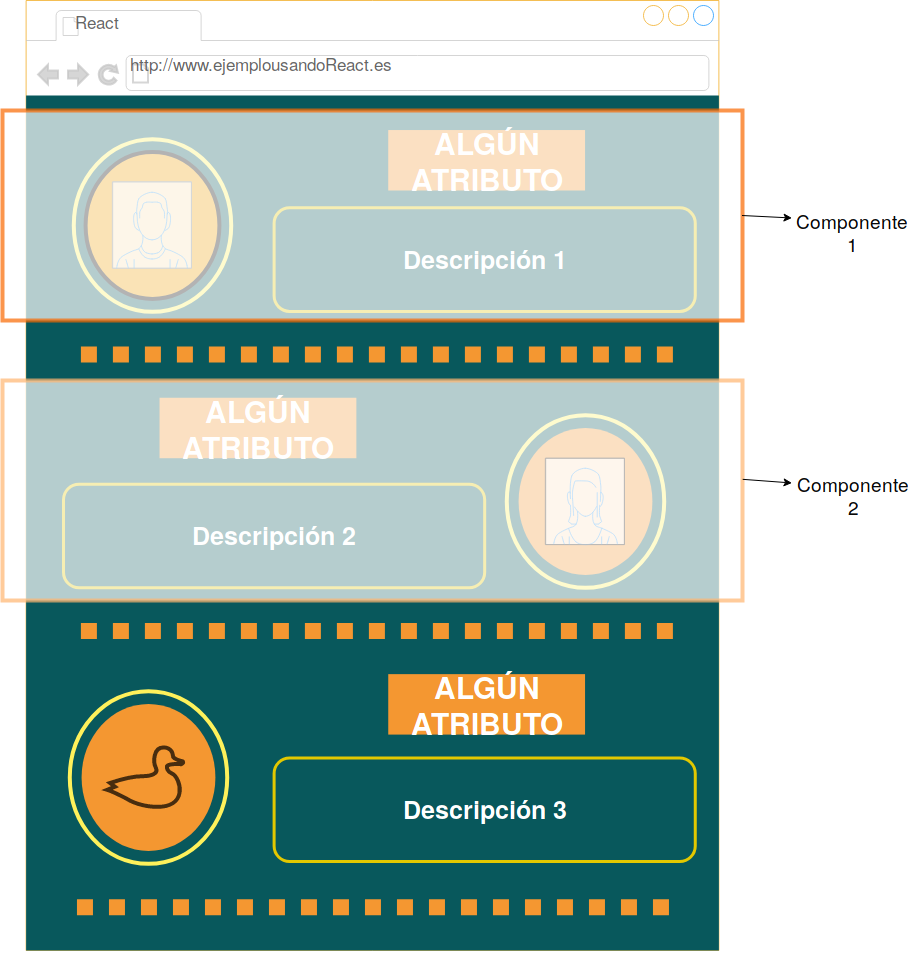
\includegraphics[width=0.5\textwidth]{react_components.png}
\caption{Componentes en React.}
\label{fig:reactComponents}
\end{center}
\end{figure}

\begin{lstlisting}[language=JavaScript,captionpos=t,caption={\textbf{\textit{Hello world} usando React.}},label={lst:reactHelloWorld}]
var HelloWorld = React.createClass({    
  render: function() {    
    return (<h1>Hello, World!</h1>);    
  }    
});    
    
ReactDOM.render(<HelloWorld/>, document.getElementById('root'));
\end{lstlisting}

\subsubsection{\textit{Backend}: Node.js}

NodeJs es un entorno de ejecución de JavaScript, es decir, un entorno que incluye todo lo necesario para ejecutar un programa que se escribe en lenguaje JavaScript. JavaScript era un lenguaje que sólo se podía ejecutar sobre un navegador, por lo que con el nacimiento de NodeJs se hace posible ejecutar una aplicación JavaScript sin necesidad de un navegador web.

NodeJs opera usando el motor de ejecución $V8$ de \textit{Chrome}. Este motor se encarga de transformar el código JavaScript en código máquina, más rápido de ejecutar. El entorno de NodeJs está conducido por eventos (véase Figura \ref{fig:nodeEventDriven}), con un modelo de entrada/salida no bloqueante (al manejar ficheros o hacer peticiones \ac{HTTP} a una \ac{API}, por ejemplo), lo que lo hace ligero y eficiente.

\begin{figure}[!h]
\begin{center}
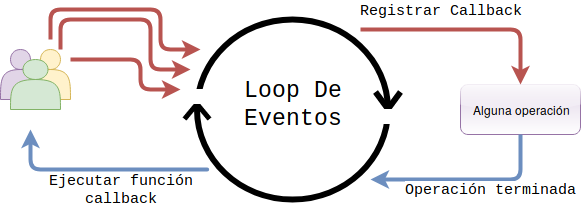
\includegraphics[width=0.5\textwidth]{node_eventdriven.png}
\caption{Modelo de ejecución conducido por eventos en NodeJs.}
\label{fig:nodeEventDriven}
\end{center}
\end{figure}

El gestor de paquetes de Node \acx{npm} proporciona una forma fácil de gestionar las dependencias en una aplicación Node. \ac{npm} permite añadir paquetes (especificando una versión determinada del mismo) a una aplicación de una forma muy sencilla. 

\begin{lstlisting}[language=JavaScript,captionpos=t,caption={\textbf{\textit{Hello world} en NodeJs.}},label={lst:nodeHelloWorld}]
console.log("Hello, world!");
\end{lstlisting}

\texttt{Express} es un \textit{framework} \cite{37} para construir aplicaciones web sobre Node.js, que proporciona un conjunto de características especialmente atractivas para el desarrollo de webs \textit{single-page} (llamadas así porque se descarga por completo la página en el cliente sin estar contínuamente haciendo peticiones al servidor, por lo que la web es más rápida), webs multipágina y webs híbridas, que mezclan ambos conceptos. 

\section{\acf{API}s}

Hoy en día muchos de los negocios son digitales. Las \ac{API}s \cite{38} se encargan de conectar los procesos de negocio, los servicios, el contenido y los datos con los socios, equipos internos y desarrolladores individuales, de una forma sencilla y segura. Las \ac{API}s se han convertido en el estándar de facto para el intercambio de datos por parte de estas empresas.

Por ejemplo, imaginemos una compañía que se dedique a la venta de productos. Un día dado, hacen una oferta de un producto en su web y esa oferta también se actualiza en su aplicación móvil. La aplicación no tiene que tratar con datos internos sobre los precios, tan sólo hace una petición a la \ac{API} (véase Figura \ref{fig:apischema}) que proporciona las ofertas de la compañía y ésta responde con la información necesaria.

\begin{figure}[!h]
\begin{center}
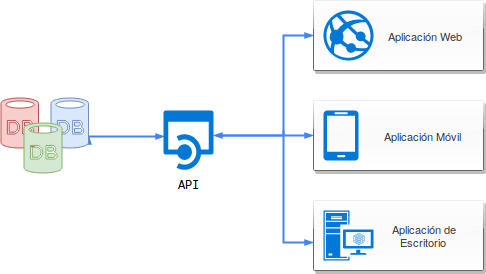
\includegraphics[width=0.5\textwidth]{api_schema.png}
\caption{Esquema básico de funcionamiento de una \ac{API}.}
\label{fig:apischema}
\end{center}
\end{figure}

La principal ventaja del uso de las \ac{API}s es el fomento de la ubicuidad. Si una empresa desarrolla una aplicación web en la que se accede a los datos a través de una base de datos tradicional y más tarde quiere desarrollar una aplicación móvil (y otras aplicaciones), el esfuerzo de desarrollo en el acceso de esos datos es mayor que mediante una \ac{API} que todas las aplicaciones compartirían, ya que tan sólo tendrían que hacer peticiones a la misma para que devolviese la información deseada.

\begin{figure}[!h]
\begin{center}
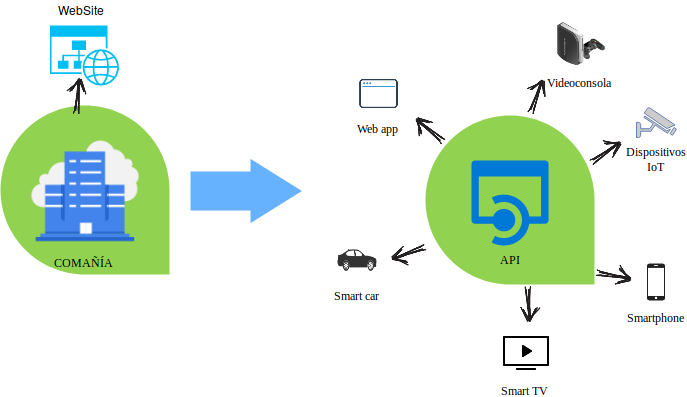
\includegraphics[width=0.5\textwidth]{api_ubicuo.png}
\caption{Ubicuidad en el uso de las \ac{API}s.}
\label{fig:apiubicuo}
\end{center}
\end{figure}

Con el crecimiento de las aplicaciones móviles, ha aumentado el uso de las \ac{API}s. Hoy en día, no resulta raro que una aplicación móvil permita registrarnos e iniciar sesión para acceder a sus servicios mediante redes sociales como \textit{Facebook}, \textit{Twitter} o \textit{Google}. Estas aplicaciones hacen uso de las \ac{API}s que dichas empresas ponen a la disposición de los desarrolladores. Normalmente, para hacer uso de una \ac{API} externa, se necesita una \textit{\ac{API} Key}. Se trata de una clave que identifica y autentica a un usuario como legítimo para usar los servicios de la \ac{API}. También se suele utilizar para tasar el uso de la \ac{API} y cobrar al usuario por el empleo de la misma.

\acx{REST} se trata de una interfaz entre sistemas que usa el protocolo \ac{HTTP} para obtener o manipular datos. En una comunicación cliente-servidor podemos usar una comunicación \ac{HTTP} para realizar la petición de datos. Este tipo de arquitectura de comunicación se denomina arquitectura \ac{REST} y es muy sencilla. Existen otro tipo de arquitecturas como puede ser \ac{SOAP}, pero su complejidad para manejar los datos es mucho mayor.

Hay que tener en cuenta que una arquitectura \ac{REST} debe cumplir ciertas propiedades y restricciones. No se pueden publicar servicios \ac{RPC} (por lo que no se puede, por ejemplo, hacer una llamada a una función expuesta por el servidor). En vez de publicar estos servicios, se publican recursos entendidos como entidades que pueden accederse de forma pública. 

\subsection{\ac{API} de \ac{AEMET}}

\acx{AEMET} \cite{39} posee una \ac{API} \ac{REST} gracias a la cual se pueden descargar de forma gratuita datos meteorológicos. Gracias a esta \ac{API} un desarrollador puede realizar consultas de una manera programada y períodica a los datos meteorológicos, con el objetivo de usarlos en la aplicación que está desarrollando. Los datos a los que un desarrollador tiene acceso son:

\begin{itemize}
\item Datos de observación, radiación y contaminación de fondo.
\item Imagenes de radar, mapas de rayos y productos derivados de satélite.
\item Climatología, valores normales y productos climatológicos.
\item Predicciones normalizadas, específicas y marítimas.
\item Mapas significativos, de análisis y previstos.
\item Avisos de fenómenos meteorológicos adversos e índices de incendios.
\end{itemize}

Para tener acceso a la \ac{API} de \ac{AEMET} es necesario obtener primero una <<\textit{\ac{API} Key}>>. Esta clave servirá para acceder al servicio que proporciona la \ac{API} y dura 90 días desde que la generación de la misma. La petición de la clave se puede realizar en la web \url{https://opendata.aemet.es/centrodedescargas/altaUsuario} y se enviará al correo que se introduzca en dicha web (véase Figura \ref{fig:aemet_apikey}). \\

\begin{lstlisting}[language=python,captionpos=t,caption={\textbf{Inventario con todas las características de todas las estaciones climatológicas.}},label={lst:aemetcode}]
from requests import request

url = "https://opendata.aemet.es/opendata/api/valores/climatologicos/inventarioestaciones/todasestaciones/"

querystring = {"api_key":"........"}
headers = { 'cache-control': "no-cache" }

response = request("GET", url, headers=headers, params=querystring)
print(response.text)
\end{lstlisting}

\begin{figure}[!h]
\begin{center}
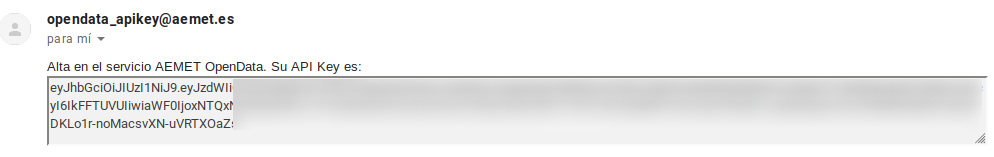
\includegraphics[width=1\textwidth]{aemet_apikey.png}
\caption{\textit{\ac{API} key} para el uso del servicio \ac{AEMET}.}
\label{fig:aemet_apikey}
\end{center}
\end{figure}

\subsection{\ac{API} de \textit{Google Maps}}
\label{apiGoogleMaps}
\textit{Google Maps} nació en febrero del año 2005 a manos de la compañía \textit{Google} \cite{40} revolucionando la forma en la que se usaban mapas en las páginas web, permitiendo a los usuarios navegar por el mapa. Las soluciones para tratar mapas antes del nacimiento de \textit{Google Maps} requerían servidores de mapas especiales, que eran muy caros. La primera versión de la \ac{API} de \textit{Google Maps} fue concebida en junio de ese mismo año.

Las localizaciones en el mundo se expresan en forma de coordenadas. Existen distintos sistemas de coordenadas, sin embargo \ac{WGS 84} es el usado por \textit{Google Maps} y también por \ac{GPS}. Las coordenadas se expresan en términos de latitud y longitud. La latitud se mide desde el sur hacia el norte y la longitud se mide desde el oeste hacia el este. En el ecuador, la latitud es 0, por lo que todo valor de latitud por debajo del ecuador (relativo al hemisferio sur) será negativo. El valor 0 de longitud se encuentra en el meridiano de \textit{Greenwich} y toda longitud al oeste de este meridiano será negativa. El formato de las coordenadas es el de dos números decimales separados por una coma. El primer número se refiere a la latitud y el segundo a la longitud.

Para usar la \ac{API} de \textit{Google Maps} es necesario obtener previamente una <<\ac{API} Key>> que se usará para hacer un seguimiento de las peticiones a la \ac{API} relacionadas con un proyecto para la facturación de los servicios. Normalmente se usará una <<\ac{API} Key>> distinta para cada uno de los proyectos que necesiten hacer uso de la \ac{API} de \textit{Google Maps}. En el Listado \ref{lst:gmaps} se puede observar el lugar en el que irá la clave de la \ac{API} (\lstinline[columns=fixed]{key=YOUR_API_KEY}). Sin esta clave, no se podrá disfrutar de los servicios de la \ac{API}.

\begin{lstlisting}[language=html,captionpos=t,caption={\textbf{Ejemplo básico del uso de la \ac{API} de \textit{Google Maps}, para visualizar en un mapa Ciudad Real.}},label={lst:gmaps}]
<!DOCTYPE html>
<html>
  ...
  <body>
    <div id="map"></div>
    <script>
      var map;
      function initMap() {
        map = new google.maps.Map(document.getElementById('map'), {
          center: {lat: 38.955 , lng: -3.98},
          zoom: 8
        });
      }
    </script>
    <script src="https://maps.googleapis.com/maps/api/js?key=YOUR_API_KEY&callback=initMap"
    async defer></script>
  </body>
</html>
\end{lstlisting}

% Local Variables:
%  coding: utf-8
%  mode: latex
%  mode: flyspell
%  ispell-local-dictionary: "castellano8"
% End:
